
\chapter{Tehtävä 1 \label{chap:Teht=0000E4v=0000E4-1}}

Tehtävässä muokataan Gorilla -pelin rakennusluokkia niin, että niihin voidaan
toteuttaa järjestelyalgoritmeja.

\section{Leveyden ja korkeuden mukainen järjestys}

\label{}

Lajittelua varten muodostetaan ensiksi Rakennus -luokkaan Comparator, niin
leveys kuin korkeusjärjestyksen muodostamiseen.

\begin{javacode}
public static Comparator<Rakennus> LeveysJärjestys = new Comparator<Rakennus>() {
	public int compare(Rakennus eka, Rakennus toka) {
		return eka.getLeveys() - toka.getLeveys();
	}
};

public static Comparator<Rakennus> KorkeusJärjestys = new Comparator<Rakennus>() {
	public int compare(Rakennus eka, Rakennus toka) {
		return eka.getKorkeus() - toka.getKorkeus();
	}
};
\end{javacode}

Jos halutaan, että Arrays.sort() -metodi järjestää rakennukset ensisijaisesti
korkeuden mukaan, niin Rakennus -luokan tulee toteuttaa Comparable -rajapinta ja
ylikirjoittaa metodi compareTo() seuraavalla tavalla:

\begin{javacode}
/**
 * Paleutetaan ensisijaisesti korkeusjärjestys, mutta jos rakennukset ovat 
 * yhtä korkeita, niin silloin palautetaan leveysjärjestys.
 */
@Override
public int compareTo(Rakennus that) {
	int korkeusjärjestys = Rakennus.KorkeusJärjestys.compare(this,that);
	return korkeusjärjestys != 0 ? 
		korkeusjärjestys : Rakennus.LeveysJärjestys.compare(this, that); 
}
\end{javacode}

Jolloin tilanteet, joissa rakennukset ovat yhtä korkeita arvioidaan rakennusten
leveyden perusteella.

\section{Järjestysnumeron esittäminen}

\label{}

Ohjelmassa järjestysnumerot voidaan piirtää rakennusten alapuolelle käyttämällä
edellisessä luvussa esiteltyä compareTo() -metodia listan järjestämisessä. Nyt
listan sort() -metodi on tosin staattinen. Rakennusten piirtämistä voidaan
helposti muokata näyttämään järjestysnumero kirjoittamalla
drawForegroundContent() -metodiin muunneltu silmukka:

\begin{javacode}
ArrayList<Rakennus> järjestettyKopio = new ArrayList<>(rakennukset);
järjestettyKopio.sort(null);

for (Rakennus r : rakennukset) {
	Rakennus skaalattu = r.skaalaa(suhdeLeveys, suhdeKorkeus);
	piirräRakennus(paikka, skaalattu);
	drawText(paikka.add(skaalattu.leveys / 2, -32), CoreColor.White,
		järjestettyKopio.indexOf(r) + "#", 24, true, true); paikka =
		paikka.add(skaalattu.leveys, 0); 
}
\end{javacode}

Silmukkaa ennen rakennusten järjestys laitetaan piirtämistä varten muistiin.
Tämä muistinkäyttö olisi järkevämpi tehdä jossain muussa luokassa, mutta koska
tässä esimerkissä rakennukset on tallennettu PiirtelyPinta -luokan sisään, niin
käytämme sitten myös PiirtelyPinta -luokkaa järjestyksen tallentamiseen.

Jotta saataisiin järjestystä vaihdettua ajon aikana GorillaPiirtopinta -luokassa
tulee myös tietää missä järjestyksessä järjestysnumero pitää esittää, joten
tallennetaan staattiseen muuttujaan käytettävä Comparator.

\begin{javacode}
public class GorillaPiirtopinta extends PiirtelyPinta {
    private final List<Rakennus> rakennukset;
    private Comparator<Rakennus> järjestys = Rakennus.KorkeusJärjestys;
    jne
}
\end{javacode}

Ja muokataan piirtämistä hiukan:

\begin{javacode}
ArrayList<Rakennus> järjestettyKopio = new ArrayList<>(rakennukset);
järjestettyKopio.sort(järjestys);

for (Rakennus r : rakennukset) {
	Rakennus skaalattu = r.skaalaa(suhdeLeveys, suhdeKorkeus);
	piirräRakennus(paikka, skaalattu);
	drawText(paikka.add(skaalattu.leveys / 2, -32), CoreColor.White,
		järjestettyKopio.indexOf(r) + "#", 24, true, true); paikka =
		paikka.add(skaalattu.leveys, 0); 
}
\end{javacode}

jossa oletusjärjestyksen (null-arvon) sijaan käytetäänkin staattiseen muuttujaan
tallennettua järjestystä (ks. rivi 2). Jäljelle jää tehdä toiminnallisuus alla
oleviin painikkeisiin niin, että järjestystä voidaan muuttaa ajon aikana.

Koska luokkarakenne ei ole erityisen eheä (edellämainittu ristiriita
piirtämiseen tarkoitetun luokan sisälle tallennettu datarakenne), niin tehdään
järjestäRakennukset() -metodi, jonka argumenttina välitetään oikea järjestys:

\begin{javacode}
void järjestäRakennukset(Comparator<Rakennus> c) {
		rakennukset.sort(c); // tullaan siirtämään seuraavassa tehtävässä pois täältä
		järjestys = c;
}
\end{javacode}

jolloin ohjelman logiikan puolella voidaan muuttaa staattista järjestystä:

\begin{javacode}
@Override
public List<Node> bottomBarContent() {
	List<Node> napit = new ArrayList<Node>(Arrays.asList(
		new Button("Järjestys #1") {
			{ setOnAction(e -> 
			appLogic.järjestäRakennukset(Rakennus.KorkeusJärjestys));
		} },
		new Button("Järjestys #2") {
			{ setOnAction(e -> 
			appLogic.järjestäRakennukset(Rakennus.LeveysJärjestys)); }
		},
		new Button("Lajittelu") {
			{ setOnAction(e -> 
			System.out.println("TODO")); }
		}
	));
	napit.addAll(basicButtons());
	return napit;
}
\end{javacode}

\section{Lajittelu ajon aikana}

\label{}

Lisätään lajittelu-painikkeelle oma metodi, joka päivittää rakennusten
järjestyksen. Tämä tehdään GorillaPiirtopinta ja GorillaLogic -luokkiin. Samalla
eritellään järjestyksen ja lajittelun käsitteet toisistaan:

\begin{javacode} 
void järjestäRakennukset(Comparator<Rakennus> c) {
		järjestys = c;
}

public void lajitteleRakennukset() {
		rakennukset.sort(järjestys);
}
\end{javacode}

jolloin nyt nappien toiminta kirjoitetaan näin:

\begin{javacode}
new Button("Järjestys #1") {
    { setOnAction(e -> 
    appLogic.järjestäRakennukset(Rakennus.KorkeusJärjestys)); }
},
new Button("Järjestys #2") {
    { setOnAction(e -> 
    appLogic.järjestäRakennukset(Rakennus.LeveysJärjestys)); }
},
new Button("Lajittelu") {
    { setOnAction(e -> 
    appLogic.lajitteleRakennukset()); }
}
\end{javacode}

Lajiteltu näkymä on esitetty kuvassa \ref{Gorillalajitelma}.

\begin{figure}
\centering 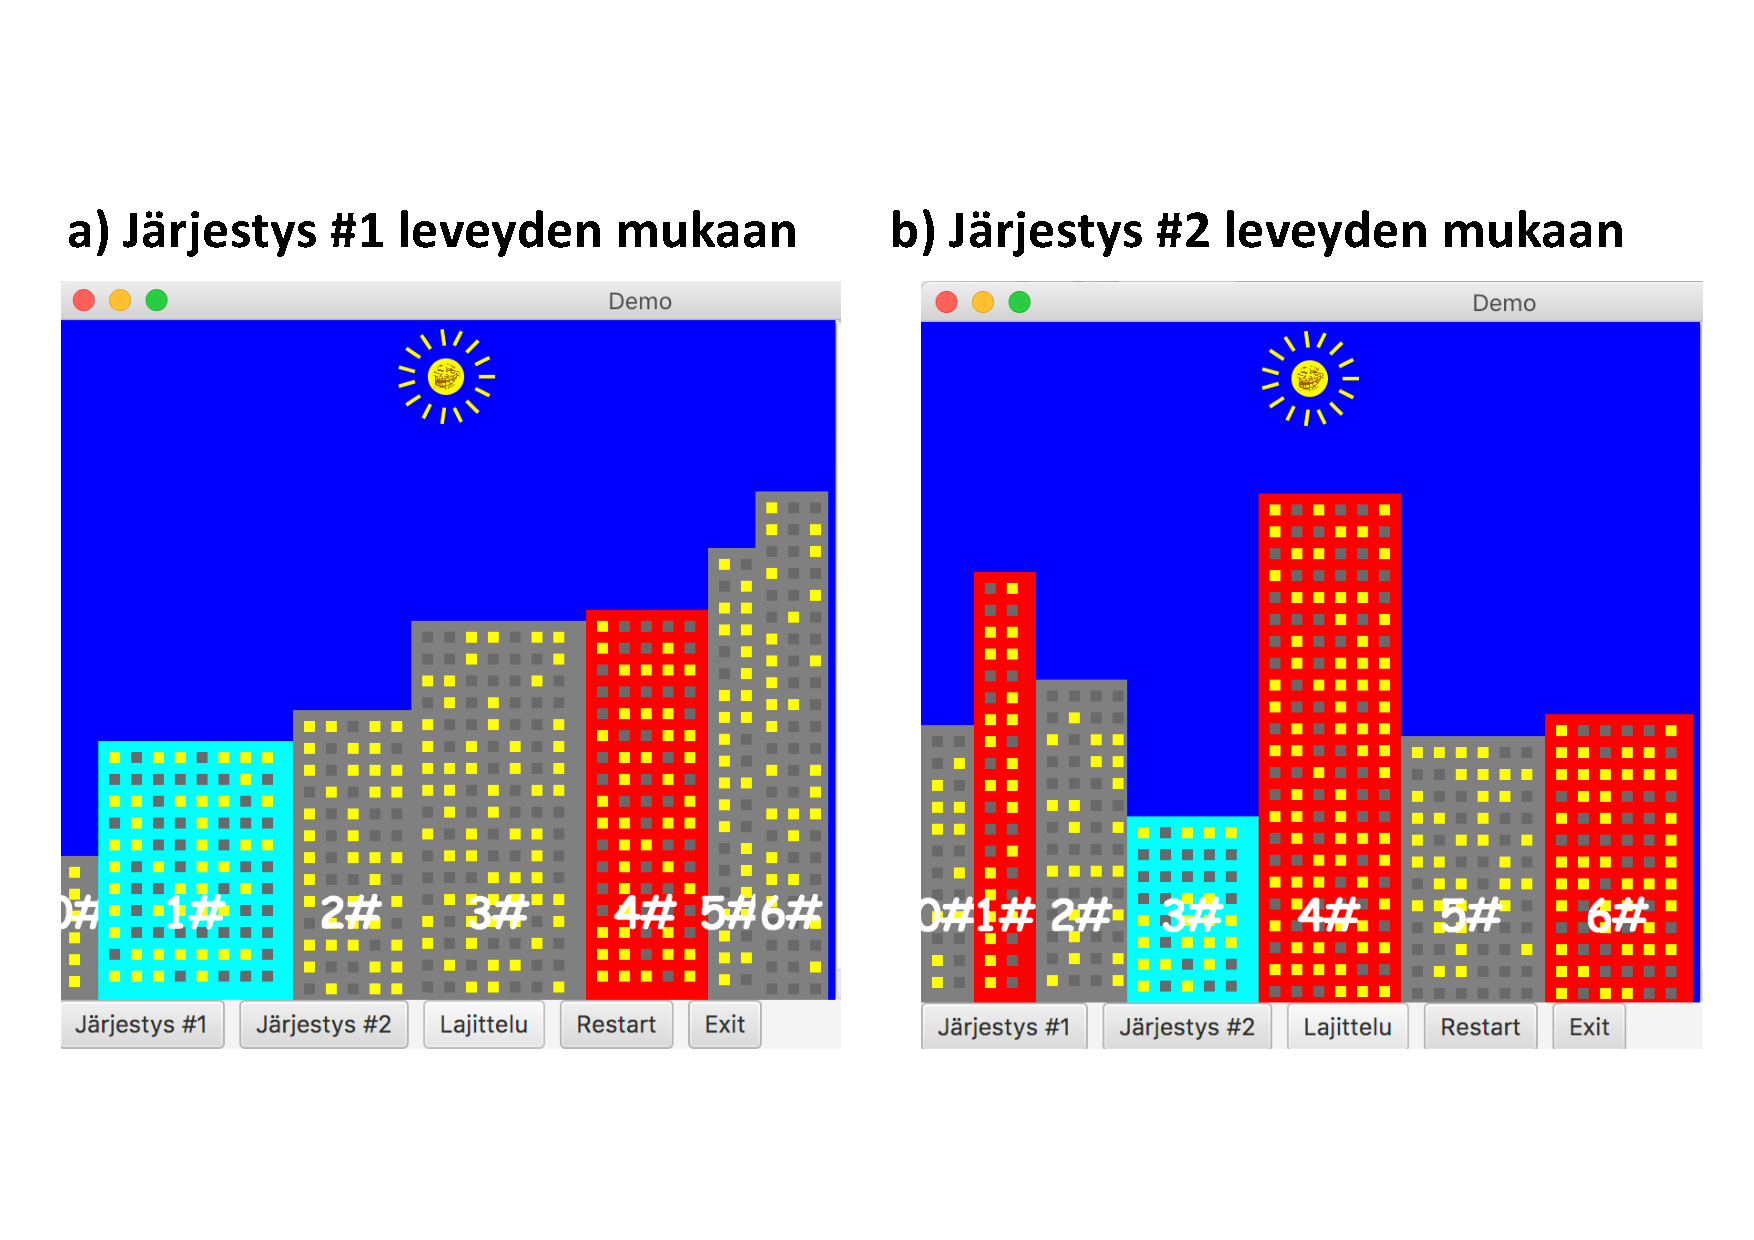
\includegraphics[width=0.5\textwidth]{kuvat/Gorillamaisema}
\caption{Lajittelunäkymä korkeus- ja leveysjärjestyksessä}
\label{Gorillalajitelma} 
\end{figure}

\section{Rakennusten sekoittaminen}

\label{}

Jos rakennukset halutaan sekoittaa silloin, kun halutaan järjestää jo
järjestyksessä olevaa listaa rakennuksista, niin tämä voidaan toteuttaa
muokkaamalla lajittelu -metodia:

\begin{javacode}
public void lajitteleRakennukset() {
	ArrayList<Rakennus> rakennuksetOld = new ArrayList<>(rakennukset);
	rakennukset.sort(järjestys);
	if ( rakennukset.equals(rakennuksetOld) ) {
		Collections.shuffle(rakennukset);
	}
}
\end{javacode}

Jolloin rakennukset sekoitetaan vain, jos muutosta järjestykseen ei tapahdu.

Tehnyt Pasi Toivanen (517487)
